\chapter{Nakamoto Consensus in Bitcoin}
\label{chpr:btc}
Bitcoin is a distributed, decentralized, peer-to-peer electronic payment system based on cryptographic proof instead of trust, allowing transactions between two counterparts without the need for a trusted third party. However, in late 2008, when the white paper was published by his inventor Satoshi Nakamoto\footnote{The name Satoshi Nakamoto is the pseudonym adopted by the creator of Bitcoin. While his identity remains a mystery, some information is known. He registered the domain bitcoin.org in August 2008 and in October 2008 he publicly released the famous white paper. In the Bitcoin's early days he participated extensively in forums and mailing lists maintaining the souce code. During the next two years other contributors slowly taken over the project maintenance and he stopped communicating, leaving a veil of mystery.} \cite{nakamoto2012bitcoin}, it lacked a formalization of the protocol and of the guarantees it claimed to provide.

\bigskip
\noindent
This chapter delves into the core innovation behind Bitcoin, i.e. \textit{Nakamoto consensus}, term that is commonly used to refer to Bitcoin's novel consensus mechanism, which allows mutually distrusting pseudonymous\footnote{Agents in the bitcoin network play under a pseudonym, that is the \textit{address} to which they receive transactions. As specified in the original white paper \cite{nakamoto2012bitcoin}, Bitcoin users are recommended to use a new address for each transaction in order to avoid that many transactions are connected to a common owner, leading anonymity.} identities to reach eventual agreement.

\bigskip
\section{Eventual Consistency}
\label{sec:eventual-consistency}
By its very nature, the Bitcoin network is subject to a type of failure called \textit{network partition}, where a network splits into at least two parts that cannot communicate with each other, often due to software bugs, incompatible protocol versions, or simply network disconnections.
Thus, Bitcoin is inherently characterized by a trade-off between \textit{consistency}, \textit{availability} and \textit{partition tolerance}. Let us be more precise.
\begin{mydef} {\bf (consistency)}.
    All nodes in the system agree on the current state of the system.
\end{mydef}
\begin{mydef} {\bf (availability)}.
    The system is operational and instantly processing incoming requests.
\end{mydef}
\begin{mydef} {\bf (partition tolerance)}.
    Partition tolerance is the ability of a distributed system to continue operating correctly even in the presence of a network partition.
\end{mydef}

\bigskip
\noindent
In practice, only two of these properties can be reached simultaneously; a theorem by Brewer proves this result.
\begin{thm} {\bf (CAP theorem)}.
    It is impossible for a distributed system to simultaneously provide consistency, availability and partition tolerance. A distributed system can satisfy any two of these but not all three.
\end{thm}
\begin{proof}
    Let us assume two nodes that share some state. The nodes belongs to different partitions, so they cannot communicate each other. Assume a request wants to update the state and contacts one of the two nodes. The node may either: 1) update its local state, resulting in a situation of inconsistent states, or 2) not update, resulting in a system no longer available for updates.
\end{proof}

\bigskip
\noindent
Recalling the Definition \ref{def:consensus} of consensus and the properties it must satisfy, a clever intuition of Nakamoto is to weaken the agreement property to hold probabilistically and not deterministically, in order to deal with an asynchronous network. In particular the aforementioned trade-off is in advantage of partition tolerance rather than consistency. In fact, state changes of the underlying transaction ledger (i.e. the blockchain), are rendered probabilistic and the decision on a specific value of the state reaches $Pr(1)$ when $\lim_{r \to \infty}$, where $r$ is the number of rounds in the consensus protocol.

\bigskip
\noindent
Therefore, we can look at Bitcoin as an example of \textit{eventual consistency}.
\begin{mydef}{\bf (eventual consistency)}
    If no new updates to the shared state are issued, then eventually the system is in a quiescent state, i.e., no more messages need to be exchanged between nodes, and the shared state is consistent.
\end{mydef}

\bigskip
\noindent
Now that we have clear in mind the consensus problem from a computer science perspective, we must move forward and study how practically Nakamoto consensus works. Starting from a brief summary of some basic Bitcoin mechanics, we will finally show how cleverly Nakamoto solves the consensus problem in Bitcoin, going through cryptography tools and game theory aspects.

\bigskip
\section{Bitcoin Design}
\label{sec:btc-design}
We already defined Bitcoin as a distributed, decentralized, peer-to-peer electronic payment system, but we lacked about defining the underlying digital asset, i.e. \textit{bitcoin}, the challenges in building it, and how the Bitcoin protocol is designed. Combining all these aspects is crucial to fully understand Nakamoto consensus.

\bigskip
\subsection{Constructing a Decentralized Digital Currency}
\label{sec:decentralized-currency}
\textit{Ownership} is the first challenge of constructing a virtual currency. Imagine units of fiat currencies, their ownership depends on their form. If these units are in the form of paper notes or metal coins, ownership is simply determined by physical possession. Else, if these units are digitally stored in a bank account, ownership is determined by possession of the credentials to spend them. But what about ownership for a decentralized virtual currency? Who maintains the ledger of credentials? How can we guarantee the integrity of that ledger? In a network like Bitcoin nodes are free to leave at any time, thus a single source of trust (a node or a group of them) cannot be given this responsibility, even if one-way functions protects credentials. A solution could be that all nodes maintain a copy of that ledger, but what about validation? Can I feasible query all the nodes? Integrity is also crucial: usually digital signatures ensure it, but reminds the nodes could act maliciously and so, can I trust the signer?

\bigskip
\noindent
Another big challenge is the so called \textit{double spending} problem. This refers to the fact that the owner of some units of digital currency could spend them more than once. With fiat currencies, granted by a central authority, this problem cannot occur. In fact the bank database is the single source of truth with regard to the deposited amount of currency. Thus, spending with f.e. an online transfer, would immediately result in the rebalancing of that account to reflect the spend. However, in a peer-to-peer decentralized network some malicious agent could try to perform a double spend taking advantage of the delay in updating the shared ledger. An example will explain better.

\begin{figure}[!htbp]
    \centering
    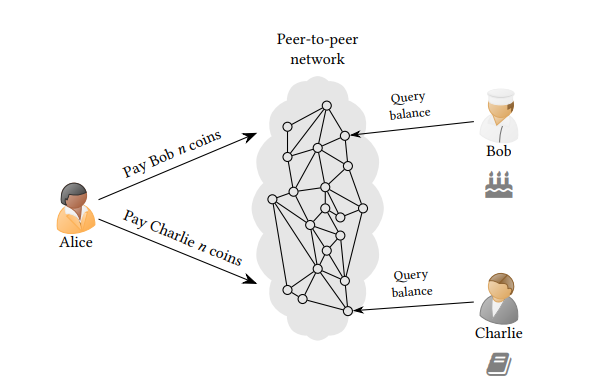
\includegraphics[width=1\linewidth]{Images/double-spending.png}
    \caption{Illustration of the double spending problem.}
    \source{\cite{Saravanan}.}
    \label{fig:double}
\end{figure}

\bigskip
\noindent
Consider the scenario described in Figure \ref{fig:double} where Alice tries to perform a double spend using some digital coins in her wallet. She would purchase a cake from Bob and a book from Charlie spending the same $n$ coins. For simplicity, let us assume that the two items cost the same, precisely $n$ units of currency. Thus, in order to finalize the purchase, both Bob and Charlie will provide Alice with their wallet addresses. Then Alice creates two different transactions, both spending the same $n$ coins, one paying Bob for the cake and the other paying Charlie for the book. The network will only accept one of them because the two transactions conflict. But there are several nodes in the network, some of which can be made to accept one of the transactions and the rest to accept the other. So Alice can transmit the transaction paying Bob to the portion of the network which Bob is connected to and the same argument holds for Charlie's transaction. Therefore, when Bob and Charlie query the balances in their private wallets they both will find a valid payment. If they provide Alice with their goods before being aware that the two transactions are conflicting, the result is that Alice has successfully performed a double spend.

\bigskip
\noindent
Nakamoto solves brilliantly the aforementioned challenges in Bitcoin combining cryptography and social incentive engineering. But first we need a brief summary of the mechanics of the protocol.

\bigskip
\subsection{Transactions and Blockchain Structure}
\label{sec:transaction-blockchain}
In Bitcoin, a coin or a \textit{bitcoin} is defined as a chain of digital signatures. Coins cannot be combined, subdivided or transferred, they can only be entirely consumed as transaction inputs (TxIn) in order to create new output coins (TxOut). Thus, a transaction output can only be in two states, \textit{spent} or \textit{unspent}. The set of current unspent coins takes the name of UTXO (Unspent Transaction Outputs). So, a \textit{transaction} assumes the role of the fundamental unit of state in the Bitcoin protocol.

\bigskip
\noindent
More precisely, each Tx\footnote{It's a common practice in Bitcoin community to abbreviate the word \textit{transaction} as Tx or sometimes TX.} output consists of an amount of bitcoins and a cryptographic puzzle, the so-called \textit{locking script}, which determines the spending conditions for that amount\footnote{Bitcoin uses a script system for transactions, called \textit{Script}. It is a simple language, Forth-like, processed from left to right using a stack. In addition, it is designed such that it guarantees all scripts will execute in a limited amount of time (i.e. it is not Touring-Complete).}. An example of such a puzzle could be a request for a digital signature which can be validated with a public key. On the other hand, a Tx input is characterized by a pointer referencing the UTXO that it consumes and an \textit{unlocking script}, the solution to the aforementioned locking script, which proves that funds in the considered transaction can be correctly spent.

\bigskip
\noindent
All the transactions, starting from the time the protocol was launched\footnote{The first block of the chain, called the \textit{genesis} block, was generated in January 2009.}, are securely recorded in a distributed ledger, shaped as a sequence of blocks, the \textit{blockchain}. In a technical cryptographic perspective, the \textit{blockchain} is a hash pointer linked list, whose aim is to be a \textit{tamper-evident} log. That is, a log data structure that stores some data (mainly transactions) allowing only to append new data onto the end of the log but, if somebody alters some earlier data then it would be easily detected. Figure \ref{fig:blockchain} provides a graphic idea of the structure.

\begin{figure}[!htbp]
    \centering
    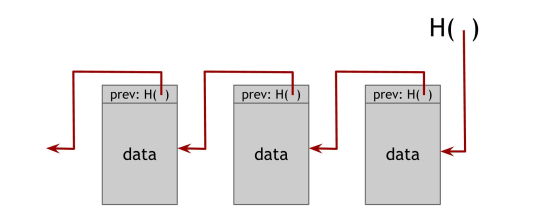
\includegraphics[width=0.9\linewidth]{Images/blockchain.png}
    \caption{Blockchain as a hash pointer linked list.}
    \label{fig:blockchain}
    \source{\cite{Narayanan:2016:BCT:2994437}.}
\end{figure}

\newpage
\bigskip
\noindent
The aforementioned \textit{tamper-evidence} property derives from cryptography, so we must introduce some primitives. But first a bit of history. The ideas behind the blockchain trace back to a paper by Haber and Stornetta in 1991 \cite{Haber91howto}. They proposed a method to \textit{timestamp} digital documents, that is a method to give an idea of when a document came into exixtance. To achieve this goal, a timestamping server receives client documents to timestamp. Then it signs the documents (one by one) together with the current time, and a special type of pointer that links to a piece of data instead of a location, pointing to the previous document. Thus, if some data is tampered, that pointer turns to be invalid. Finally the timestamping server issues a certificate containing such information. Therefore, it is clear that each document's certificate ensures the integrity of the previous document.

\subsection{Hash Functions}
\label{sec:hash}
The more the world becomes digital, the more we need information security. Cryptography mixes advanced mathematical and computer science techniques to provide confidentiality, data integrity, authentication and non-repudiation.

\bigskip
\noindent
A \textit{hash function} is a particular mathematical function that maps an arbitrary length input message into a short, fixed-length bit string, usually called \textit{digest} or \textit{hash value}. Hash functions can be seen as a digital fingerprint of a message, i.e. a unique representation of a message.

\begin{mydef}
    \label{def:hash}
	A function $h : \{ 0, 1 \} ^* \rightarrow \{ 0, 1 \} ^n $ is a hash function if it is computable in polynomial time in the length of the input.
\end{mydef}

\bigskip
\noindent
This definition lacks of security arguments. There are three main properties that hash functions need to possess in order to provide security:
\begin{mydef}
	\label{def:hash-prop}
	Let $h$ be a hash function, the following properties may hold:
	\begin{itemize}
		\item preimage resistance (one-wayness): given $h(x)$ it is not feasible to compute $x$;
		\item second-preimage resistance (weak collision resistance): given $x$ it is not feasible to compute $y$ s.t. $x \neq y$, $h(x)=h(y)$;
		\item collision resistance (strong collision resistance): it is not feasible to find $x, y$ s.t. $x \neq y$, $h(x)=h(y)$.
	\end{itemize}
\end{mydef}

\bigskip
\noindent
A hash function that fulfills the preimage resistance property \textit{hides} the input, so one cannot derive a matching message from a hash value. A second-preimage resistant hash function prevents that, given a message, one can find another message that produces the same output once hashed. Unfortunately such a property cannot exist in theory, due to the so-called \textit{pigeonhole principle}\footnote{Formally this principle takes the name of \textit{Dirichlet's drawer principle}, but it is commonly referred to as the \textit{pigeonhole principle}.}. Suppose to be the owner of 100 pigeons but in your pigeon loop are only 99 holes, at least one pigeonhole will be occupied by 2 birds. The same argument holds for hash functions. Since the output of a hash function has a fixed bit length, say $n$ bits, there exist only $2^{n}$ possible output values. However the length of input values is arbitrary, resulting in an infinite number of possible inputs. Thus, weak collision can occur in theory. Fortunately, given today's computers, an output length of $n=80$ bits is sufficient to resist an analytical attack, that is, given $x$ and $h(x)$ one wants to construct $y$ such that $h(y)=h(x)$. To sum up, collisions do exist, but they are \textit{unfeasible}. Finally, the strong collision resistance property refers to the problem of finding two messages that generate the same hash value. With an output length of $n=80$ bits as before, producing $2^{80}$ possible values, one may think that finding two inputs generating the same output would require around $\frac{2^{80}}{2}$, a half of the possible values. That's completely wrong, due to the \textit{birthday paradox}, a powerful cryptographic tool which deserves a formal definition.
\begin{mydef} {\bf (birthday paradox)}.
    The birthday paradox concerns the probability that, given a set of $n$ randomly chosen people, some pair of them will have the same birthday.
\end{mydef}

\bigskip
\noindent
The correct approach to solve this problem is to compute the probability of two people \textit{not} having the same birthday:
$$P(\text{2 people not colliding}) = \left(1-\frac{1}{365} \right).$$
If a third person is joining:
$$P(\text{3 people not colliding}) = \left(1-\frac{1}{365} \right) \cdot \left(1-\frac{2}{365} \right).$$
Hence, the probability for $t$ people having no birthday collision is given by:
$$P(\text{$t$ people not colliding}) = \left(1-\frac{1}{365} \right) \cdot \left(1-\frac{2}{365} \right) \dotsm \left(1-\frac{t-1}{365} \right).$$
Then, making some simple calculations, it turns out that it only requires 23 people to have a probability of about 0.5 for a birthday collision:
\begin{equation*}
\begin{split}
    P(\text{at least one collision}) &= 1 - P(\text{no collision}) \\
            &= \left(1-\frac{1}{365} \right) \cdot \left(1-\frac{2}{365} \right) \dotsm \left(1-\frac{23-1}{365} \right) \\
            &= 0.507 \approx 50 \%.
\end{split}
\end{equation*}
The search of a collision for a hash function is exactly the same problem as the birthday problem, obviously with different parameters. Again, let $n$ be the output length in bits, thus resulting in $2^{n}$ possible output values. Here, the probability of no collisions among $t$ hash values is:
\begin{equation*}
\begin{split}
    P(\text{no collision}) &= \left(1-\frac{1}{2^{n}} \right) \cdot \left(1-\frac{2}{2^{n}} \right) \dotsm \left(1-\frac{t-1}{2^{n}} \right) \\
            &= \prod\limits_{i=1}^{t-1} \left(1-\frac{i}{2^{n}} \right) \\
            &\approx \prod\limits_{i=1}^{t-1} e^{- \frac{i}{2^{n}}} \\
            &\approx e^{- \frac{t(t-1)}{2\cdot 2^{n}}}.
\end{split}
\end{equation*}
Remind that we want to find how many messages are required to find a collision. Let $\lambda$ be the probability of at least one collision:
$$\lambda \approx 1 - e^{- \frac{t(t-1)}{2^{n+1}}}.$$
Solving for $t$ and observing that, since in practice $t>>1$, it holds that $t^{2}\approx t(t-1)$ we obtain:
\begin{equation}
    \label{eq:collision}
    t\approx 2^{(n+1)/2} \sqrt{\ln{\left(\frac{1}{1-\lambda}\right)}}.
\end{equation}
The main takeaway of the result obtained in Equation \ref{eq:collision} is that the number of messages needed to find a collision of hash values is proportional to the square root of the number of possible output values.

\begin{myexample}
	SHA256\textup{\footnote{SHA256 belongs to the SHA2 family. Nowadays SHA3 family is available, even more secure.}} (Secure Hash Algorithm) is the hash function the Bitcoin protocol is built upon. It produces a 256 bit output digest and, at the moment, it is considered to satisfy all the properties described in Definition \ref{def:hash-prop}.
	Moreover, SHA256 could be thought as a random oracle, a fixed input will provide always the same output, since hash functions are deterministic, but the outputs corresponding to new inputs are indistinguishable from a uniform distribution. Thus, a small perturbation in the input string will result in a completely different digest.
	\begin{verbatim}
	SHA256("I love you")  = c33084feaa65adbbbebd0c9bf292a26ffc6
	                        dea97b170d88e501ab4865591aafd
	SHA256("I love you!") = c22fe0282c7b45b0926fb3e33efd375a5e1
	                        95c4c838c96075e3877b2ac2b7911
	\end{verbatim}
\end{myexample}

\subsection{Mining \& Proof of Work}
\label{sec:mining-pow}
The Bitcoin blockchain is a public distributed ledger of transactions. Being public means that anyone should be allowed to add transactions to the blockchain. However, we already saw that in a peer-to-peer asynchronous network like this, some nodes are byzantine and could be malevolent, trying to perform doublespends, which can result in an inconsistent state since the validity of transactions depends on the order in which they arrive, not the same for all nodes. Thus, if doublespends are not resolved, the shared state diverges. Hence, we need a mechanism to resolve conflicting transactions, the so-called \textit{proof-of-work}\footnote{The idea of \textit{proof-of-work} is taken from Adam Back's Hashcash \cite{Back02hashcash-}, a scheme to combat email spam proposed in 1997.}, in order to append only valid blocks to the blockchain.

\begin{mydef}{\bf (proof-of-work)}.
    \label{def:pow}
    The proof-of-work (pow) is a mechanism allowing a party to prove to another party that a certain amount of computational power has been used for a period of time. A function $F_{d}(c,x) \rightarrow \{true,false\}$, where the difficulty $d$ is a positive number, while the challenge $c$ and the nonce $x$ are usually strings of bits, is a pow function if it satisfies the following properties:
    \begin{enumerate}
        \item if $d$, $c$ and $x$ are given, $F_{d}(c,x)$ is fast to compute.
        \item For fixed $c$ and $d$, finding $x$ s.t. $F_{d}(c,x) = true$ is computationally hard but feasible. In addition, the difficulty $d$ serves to adjust the time to find that $x$.
    \end{enumerate}
\end{mydef}

\bigskip
\noindent
However, the proof-of-work mechanism by itself does not fully solve the double-spending problem. But, if correctly used, it makes the blockchain tamper-resistant, thus extremely hard and expensive to rewrite. We will see how the proof-of-work is shaped in Bitcoin just in a while, inside the explanation of the network behaviour.

\bigskip
\noindent
The clever intuition of Nakamoto in resolving doublespends is to incentivize network nodes to behave honestly, checking for and rejecting fraudolent transactions. The procedure by which new blocks are added to the blockchain while ensuring that they contain only valid transactions is called \textit{mining}. In addition, this procedure controls the rate of generation of new bitcoins. Before delving into the details of the mining procedure, we have to show a summary algorithm of the Bitcoin network behaviour, presented in the original white paper by Nakamoto \cite{nakamoto2012bitcoin}.

\begin{algorithm}
	\caption{Bitcoin network behaviour}
	\label{alg:btc-network}
	\begin{algorithmic}[1]
		\State New transactions are broadcast to all nodes.
		\State Each node collects new transactions into a block.
		\State Each node works on finding a difficult proof-of-work for its block.
		\State When a node finds a proof-of-work, it broadcasts the block to all nodes.
		\State Nodes accept the block only if all transactions in it are valid and not already spent.
		\State  Nodes express their acceptance of the block by working on creating the next block in the chain, using the hash of the accepted block as the previous hash.
	\end{algorithmic}
\end{algorithm}

\bigskip
\noindent
Taking advantage of the main steps of the Bitcoin network behaviour described in Algorithm \ref{alg:btc-network}, we can proceed to define the mining procedure as a sequence of steps:

\begin{enumerate}
    \item People performing bitcoin transactions will broadcast them onto the network. Such transactions will held in the \textit{mempool} (memory pool), that is a collection of pending transactions, before being included in a block. Each node of the network operate its own mempool, with its own unique size (typically MB).
    \item Some special nodes, called \textit{miners}, collect some of these transactions into a \textit{candidate block}, which could be different for each miner, composed by a \textit{block header} and a list of transactions. The first transaction in the block is called \textit{coinbase transaction}. This special transaction has a dummy input, called \textit{coinbase}, with no references to parent TxOut, and creates new bitcoins from nothing. In addition, each transaction includes a small \textit{fee}, as the difference between inputs and outputs. Finally, the \textit{block header} consists of the following fields:
    \begin{itemize}
        \item A block version number.
        \item The double SHA256 of the previous block header.
        \item The \textit{merkleroot}\textup{\footnote{A \textit{merkleroot} is the root of a \textit{merkle tree} as presented in Definition \ref{def:merkle}.}} of all transactions in that block.
        \item The block generation time (Unix epoch time) according to the miner.
        \item An encoded version (nBits) of the target threshold this block header hash must be less than or equal to.
        \item The nonce used to effectively mine that block.
    \end{itemize}
    \item The sum of the transaction fees included in all regular transactions, plus the bitcoins generated in the coinbase transaction is called \textit{block reward}\textup{\footnote{The number of bitcoins generated by the coinbase transaction is determined by a subsidy schedule that is part of the protocol. Started with 50 bitcoins for every block, it halves every 210000 blocks (about 4 years, considering an average of a block per 10 minutes). Nowadays it consists of 12.5 bitcoins. Due to this halving, the total amount of bitcoins never exceeds 21 million of units, making this asset scarce by nature.}} and it is collected by the block's miner, allowing it to mint new coins. These economic incentives make Bitcoin a very expensive network, but they trigger a virtuous cycle\footnote{In an economic perspective, scarcity increases bitcoin market price.}, encouraging nodes to behave honestly competing to append valid blocks to the blockchain, making it almost immutable. So, each miner will compete to find that specific \textit{nonce} which verifies the Bitcoin proof-of-work. More precisely, recalling Definition \ref{def:pow}:
    
    \begin{mydef}{\bf (Bitcoin proof-of-work)}.
        \label{def:btc-pow}
        The Bitcoin proof-of-work consists of finding a special number $x$ called nonce s.t. the double SHA256 of the candidate block header falls below a given threshold\textup{\footnote{More precisely, the difficulty $d$ is calculated as: $d=\frac{\text{difficulty\_1\_target}}{\text{current\_target}}$. Traditionally, the \textit{difficulty\_1\_target} represents a hash where the leading 32 bits are zero and the rest are one, known as \textit{pool difficulty}, or \textit{pdiff}. Thus, the threshold value appears as $\frac{2^{224}}{d}$ and not $\frac{2^{256}}{d}$. In addition, the mining threshold is adaptively adjusted every 2016 blocks to achieve an average goal of a block 10 minutes (i.e. every 2 weeks).}}:
        $$F_{d}(c,x) \rightarrow \text{SHA256}(\text{SHA256}(\underbrace{... \| \text{prev\_block\_header\_hash} \| ... \| x}_{\text{Candidate Block Header}})) < \frac{2^{224}}{d}.$$
    \end{mydef}
    
    \item The miner who first finds such a nonce will broadcast his own candidate block to the network. If all the transactions in that block pass the validity check, it is appended to the miner's local copy of the blockchain. Other nodes express their acceptance of the block by working on creating a new block using the hash of the accepted block as the previous hash. However, this is not the end of the story. It is possible that two miners mine their respective candidate blocks almost at the same time and, due to connection lag, they broadcast their blocks before being aware one of the other. This situation leads to a chain \textit{fork}, that is two possible valid chains, at least for the moment. The solution to this type of problem is achieved by the \textit{proof-of-work consensus}, i.e., in favor of the chain which required the most computational work\footnote{That is, with the majority of the network total hash rate working on it.} to produce.

\end{enumerate}

\bigskip
\noindent
We set the basis for the very hearth of this thesis work, that is \textit{notarization} of digital documents with the Bitcoin blockchain. In Chapter \ref{chpr:notarization} we will study what a \textit{timestamp} on the blockchain is, introducing \textit{OpenTimestamps}, an open-source project whose aim is to be a standard for blockchain notarization. Then, in Chapter \ref{chpr:project} we will delve into the details of a project in which the author, in cooperation with DGI (Digital Gold Institute) and ANIA (Associazione Nazionale fra le Imprese Assicuratrici), built a fully operating timestamping service, modifying and extending the \textit{OpenTimestamps} protocol.